\documentclass[degree=master,tocarialchapter]{thuthesis}
% 选项
%   degree=[bachelor|master|doctor|postdoctor], % 必选,学位类型
%   language=[chinese|english], % 可选(默认:chinese),论文的主要语言
%   secret,                % 可选(默认:关闭),是否有密级
%   tocarialchapter,       % 可选(默认:关闭),章目录中使用黑体(这项表示同时打开下面两项)
%   tocarialchapterentry,  % 可选(默认:关闭),单独控制章标题在目录中使用黑体
%   tocarialchapterpage,   % 可选(默认:关闭),单独控制章页码在目录中使用黑体

% 所有其它可能用到的包都统一放到这里了,可以根据自己的实际添加或者删除。
\usepackage{thuthesis}
\usepackage{pdfpages}
\usepackage{listings}
\usepackage{color}

\definecolor{dkgreen}{rgb}{0,0.6,0}
\definecolor{gray}{rgb}{0.5,0.5,0.5}
\definecolor{mauve}{rgb}{0.58,0,0.82}

\lstset{ %
  language=Octave,                % the language of the code
  basicstyle=\footnotesize,           % the size of the fonts that are used for the code
  numbers=left,                   % where to put the line-numbers
  numberstyle=\tiny\color{gray},  % the style that is used for the line-numbers
  stepnumber=1,                   % the step between two line-numbers. If it's 1, each line 
                                  % will be numbered
  numbersep=5pt,                  % how far the line-numbers are from the code
  backgroundcolor=\color{white},      % choose the background color. You must add \usepackage{color}
  showspaces=false,               % show spaces adding particular underscores
  showstringspaces=false,         % underline spaces within strings
  showtabs=false,                 % show tabs within strings adding particular underscores
  frame=single,                   % adds a frame around the code
  rulecolor=\color{black},        % if not set, the frame-color may be changed on line-breaks within not-black text (e.g. commens (green here))
  tabsize=2,                      % sets default tabsize to 2 spaces
  captionpos=b,                   % sets the caption-position to bottom
  breaklines=true,                % sets automatic line breaking
  breakatwhitespace=false,        % sets if automatic breaks should only happen at whitespace
  title=\lstname,                   % show the filename of files included with \lstinputlisting;
                                  % also try caption instead of title
  keywordstyle=\color{blue},          % keyword style
  commentstyle=\color{dkgreen},       % comment style
  stringstyle=\color{mauve},         % string literal style
  escapeinside={\%*}{*)},            % if you want to add LaTeX within your code
  morekeywords={*,...}               % if you want to add more keywords to the set
}


% 定义所有的图片文件在 figures 子目录下
\graphicspath{{figures/}}

% 可以在这里修改配置文件中的定义。导言区可以使用中文。
% \def\myname{薛瑞尼}

\begin{document}

%%% 正文部分
\mainmatter

\chapter{计划书}
\label{cha:intro}
计划书中包含目标阐述、关键问题、具体任务和具体方案。

\section{目标阐述}
红外遥控是利用近红外光进行数据传输的一种控制方式。
近红外光波长0.76um-1.5um,红外遥控收发器件波长一般为0.8um-0.94um,
具有传输效率高,成本低,电路实现简单,抗干扰强等特点,在家用电器上被广泛使用。
此处设计一个\textbf{红外发射接收器与红外接收器,
能够实现通过按按钮而发出不同的红外波段,以达到控制的功能。}


\section{关键问题}
1. 按按钮发出不一样的红外波段

2. 红外发射和接收稳定,不易受外界波段的干扰

3. 具有可移植接口,方便进一步开发 

\section{具体任务}
1. 通过开关控制阻值,以实现不同的射频

2. 加上滤波和放大,以减少外界波段的干扰

3. 采取模块化设计,留有接口

\section{具体方案和关键技术}
详细解释了选用的芯片和原理。

\subsection{NE555}
使用NE555产生红外光线。因为NE555时基电路(集成电路)性价比高,
且价格低廉,外围元件少,根据应用需要可设计不同功能,应用十分广泛。

由NE555芯片手册可知,\textbf{通过控制RA和RB的比例即可控制频率和占空比}。
\begin{figure}[H] % use float package if you want it here
  \centering
  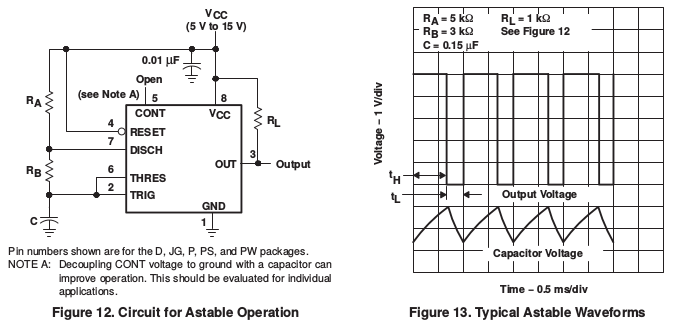
\includegraphics[width=0.8\textwidth]{1.png}
  \caption{NE555芯片手册}
  \label{fig:xfig1}
\end{figure}
比方说:使用NE555产生38kHz, 占空比为1/3的方波信号。

产生方波的频率 = 0.693((RA+2RB)*C) ,占空比 = RB/(RA+2RB)


因为红外发射管最佳的占空比是1/3,C一般为0.01uF,所以计算之后RA = RB =1.2k

此处,由于我们需要控制发射频率,因此我们把RA变成可调的电阻。

\subsection{光电二极管}
接收我们使用光电二极管用于接收产生的红外信号。
光电二极管是一种能够将光根据使用方式,转换成电流或者电压信号的光探测器。
管芯常使用一个具有光敏特征的PN结,对光的变化非常敏感,具有单向导电性,
而且光强不同的时候会改变电学特性,因此,可以\textbf{利用光照强弱来改变电路中的电流}。

\subsection{BC848B和2SC1815三极管}
使用此两款三极管以用于放大和解调。
\chapter{原理图}
\label{cha:china}
包括项目原理图和电路原理图

\section{项目原理图}
\begin{figure}[H] % use float package if you want it here
  \centering
  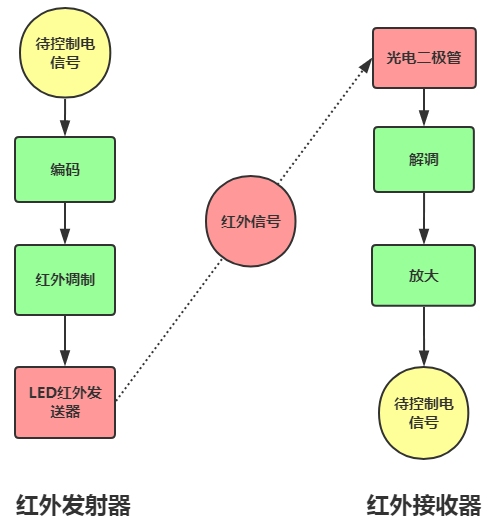
\includegraphics[width=0.7\textwidth]{2.png}
  \caption{项目原理图}
  \label{fig:xfig1}
\end{figure}
无线遥控器的原理就是发射机把控制的电信号\textbf{先编码,
然后再调制},红外调制或者无线调频、调幅,转换成无线信号发送出去。

接收机收到载有信息的无线电波\textbf{接收,放大,解码},得到原先的控制电信号,
把这个电信号再进行功率放大用来驱动相关的电气元件,实现无线的遥控。


\section{线路原理图}
\subsection{红外发射线路原理图}
\begin{figure}[H] % use float package if you want it here
  \centering
  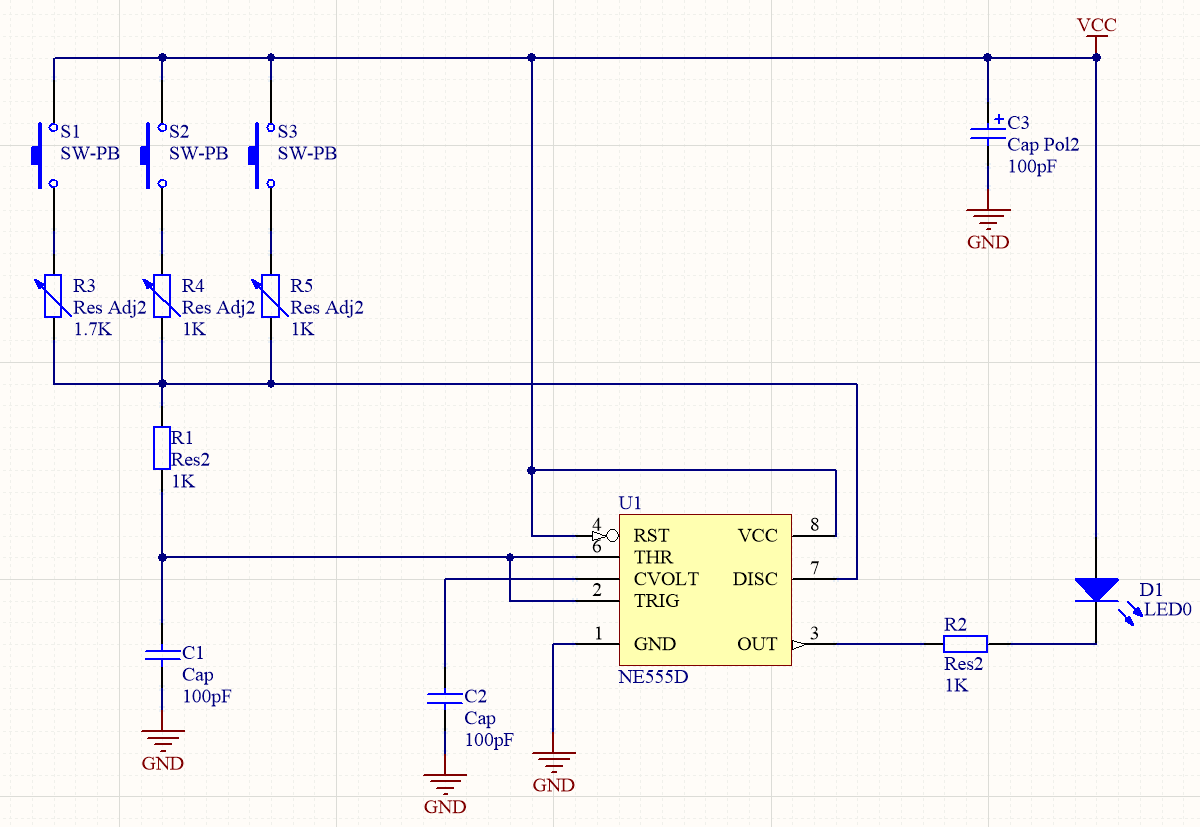
\includegraphics[width=1\textwidth]{3.png}
  \caption{红外发射线路原理图}
  \label{fig:xfig1}
\end{figure}
红外发射电路采用NE555接成振荡电路,如图所示。
振荡频率由SA1~SA3开关控制,改变开关位置,
即改变接入振荡电路的电阻RP1~RP3,调节RP1~RP3,
可以调节每一通道的具体频率。振荡脉冲由3号引脚输出,
驱动红外发光二极管发射红外光,即实现了用振荡脉冲对红外光的调制。

\subsection{红外接收线路原理图}
\begin{figure}[H] % use float package if you want it here
  \centering
  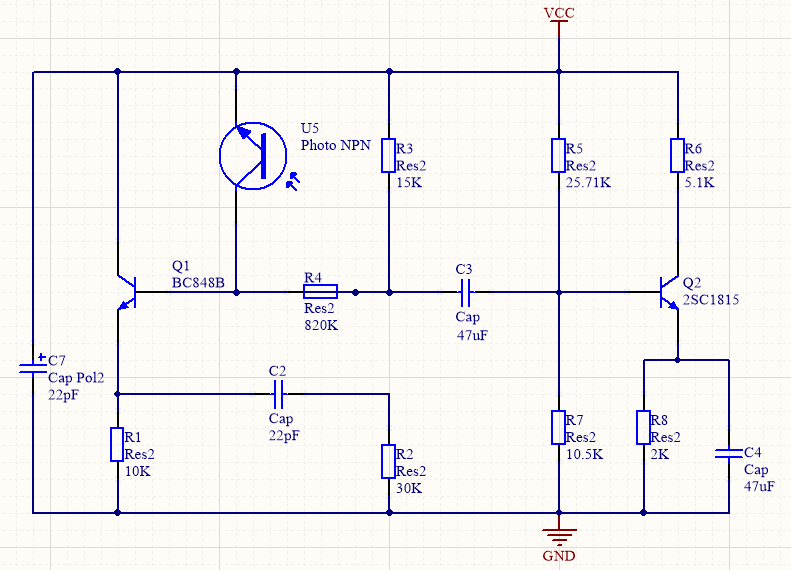
\includegraphics[width=1\textwidth]{3-2.png}
  \caption{红外接收线路原理图}
  \label{fig:xfig1}
\end{figure}
利用光电二极管接收上述红外发射电路发射的红外线,
利用光照强弱来改变电路中的电流,
通过BC848B和2SC1815三极管的放大和解调,输出得到期望的电压

\chapter{仿真}
\label{cha:intro}
在Multisim中,依据电路原理图搭建电路进行仿真测试
\section{红外发射Multisim仿真电路}
\begin{figure}[H] % use float package if you want it here
    \centering
    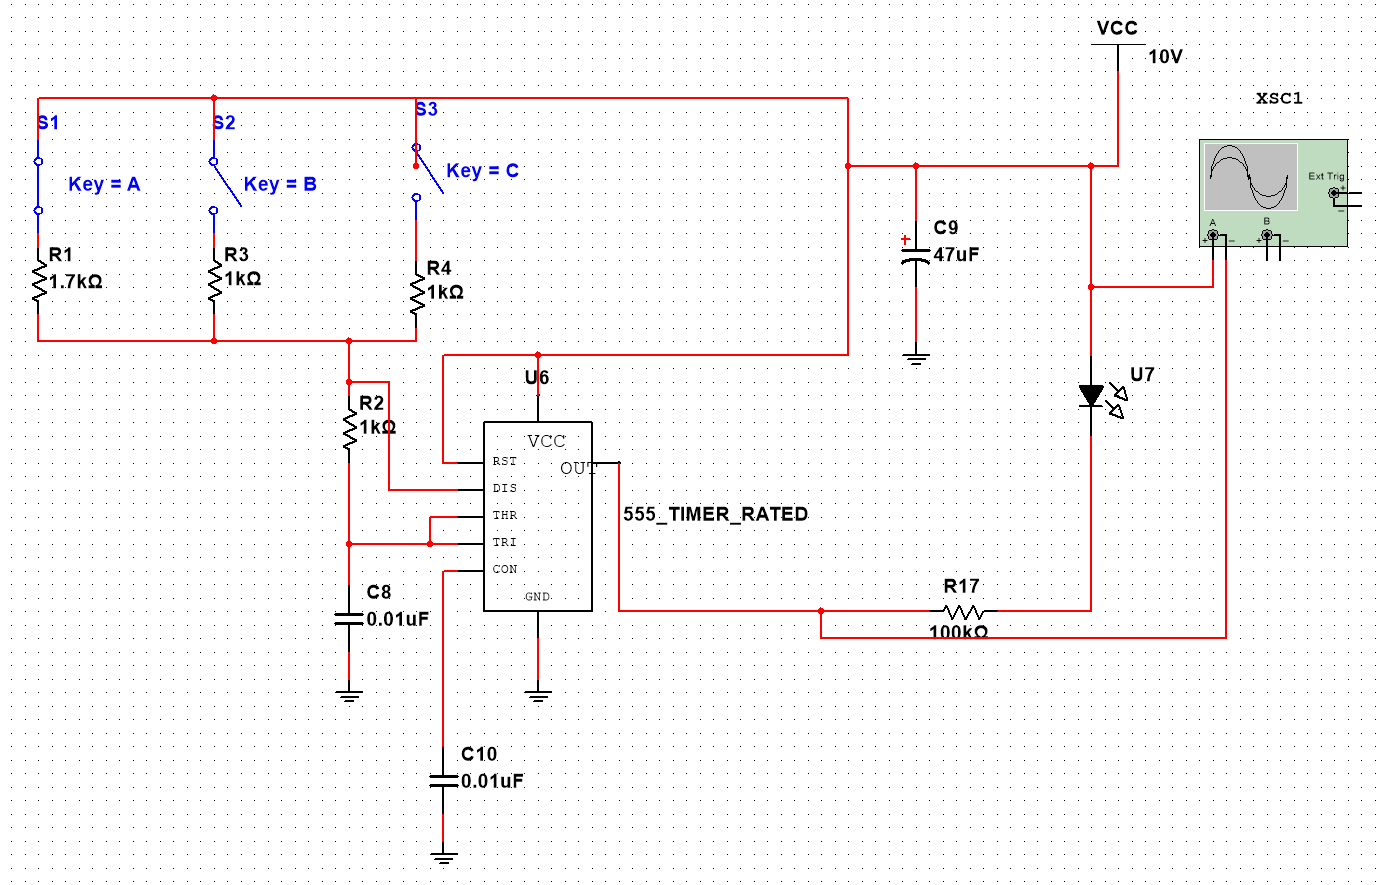
\includegraphics[width=1\textwidth]{4-1.png}
    \caption{红外发射Multisim仿真电路}
    \label{fig:xfig1}
\end{figure}

参数分析:

此处,我们使得RB为1k,为了产生使用NE555产生38kHz的方波信号。

由下式可知:

频率 = 0.693((RA+2RB)*C) 
占空比 = RB/(RA+2RB)

将RB=1k,C=0.01u带入得到

RA=1.7,因此我们需要1.7k的电阻。

此时输出的期望信号为38kHz、26.4\%占空比的方波。

~\\

其中U7为发光二极管,其参数如下:
\begin{figure}[H] % use float package if you want it here
    \centering
    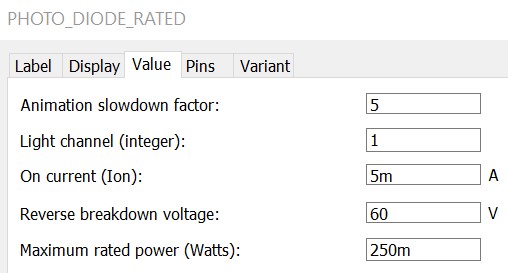
\includegraphics[width=0.5\textwidth]{4-2.png}
    \caption{U7参数}
    \label{fig:xfig1}
 \end{figure}
 ~\\

测量其输出电压波形如下:
\begin{figure}[H] % use float package if you want it here
    \centering
    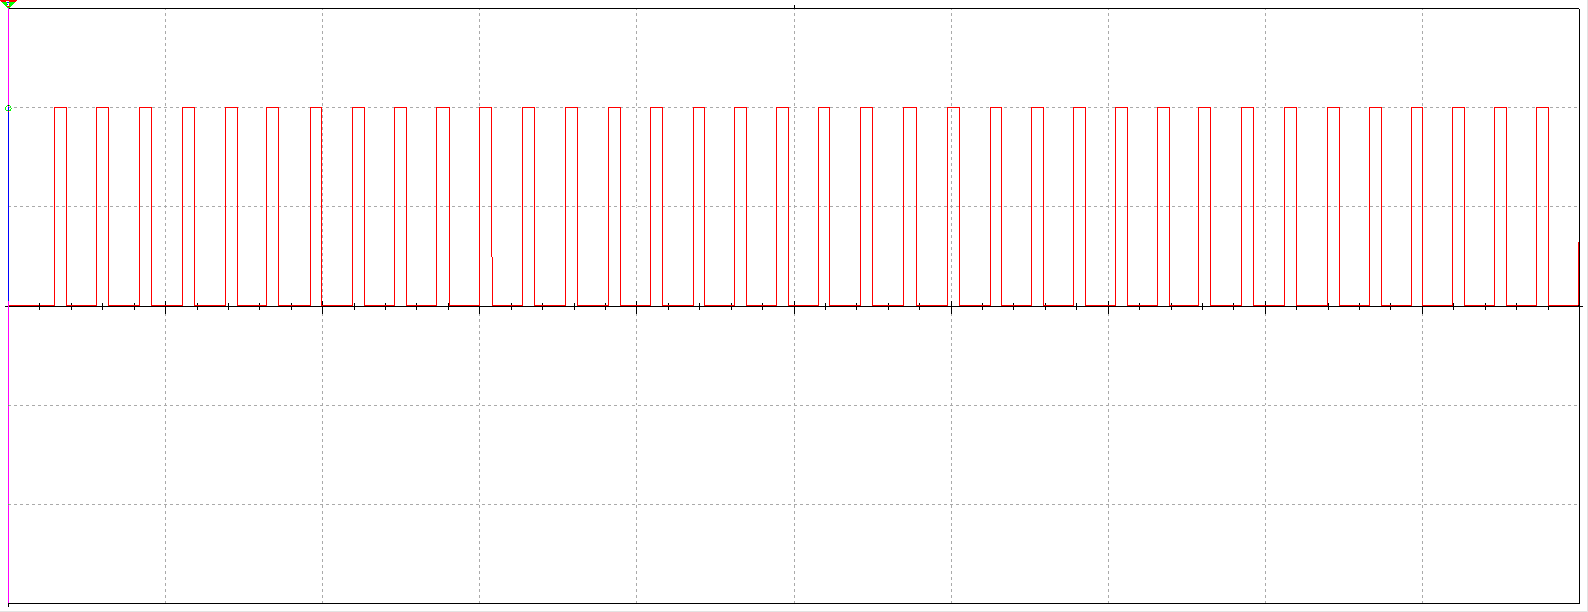
\includegraphics[width=0.8\textwidth]{4-3.png}
    \caption{红外发射整体波形}
    \label{fig:xfig1}
\end{figure}
\begin{figure}[H] % use float package if you want it here
    \centering
    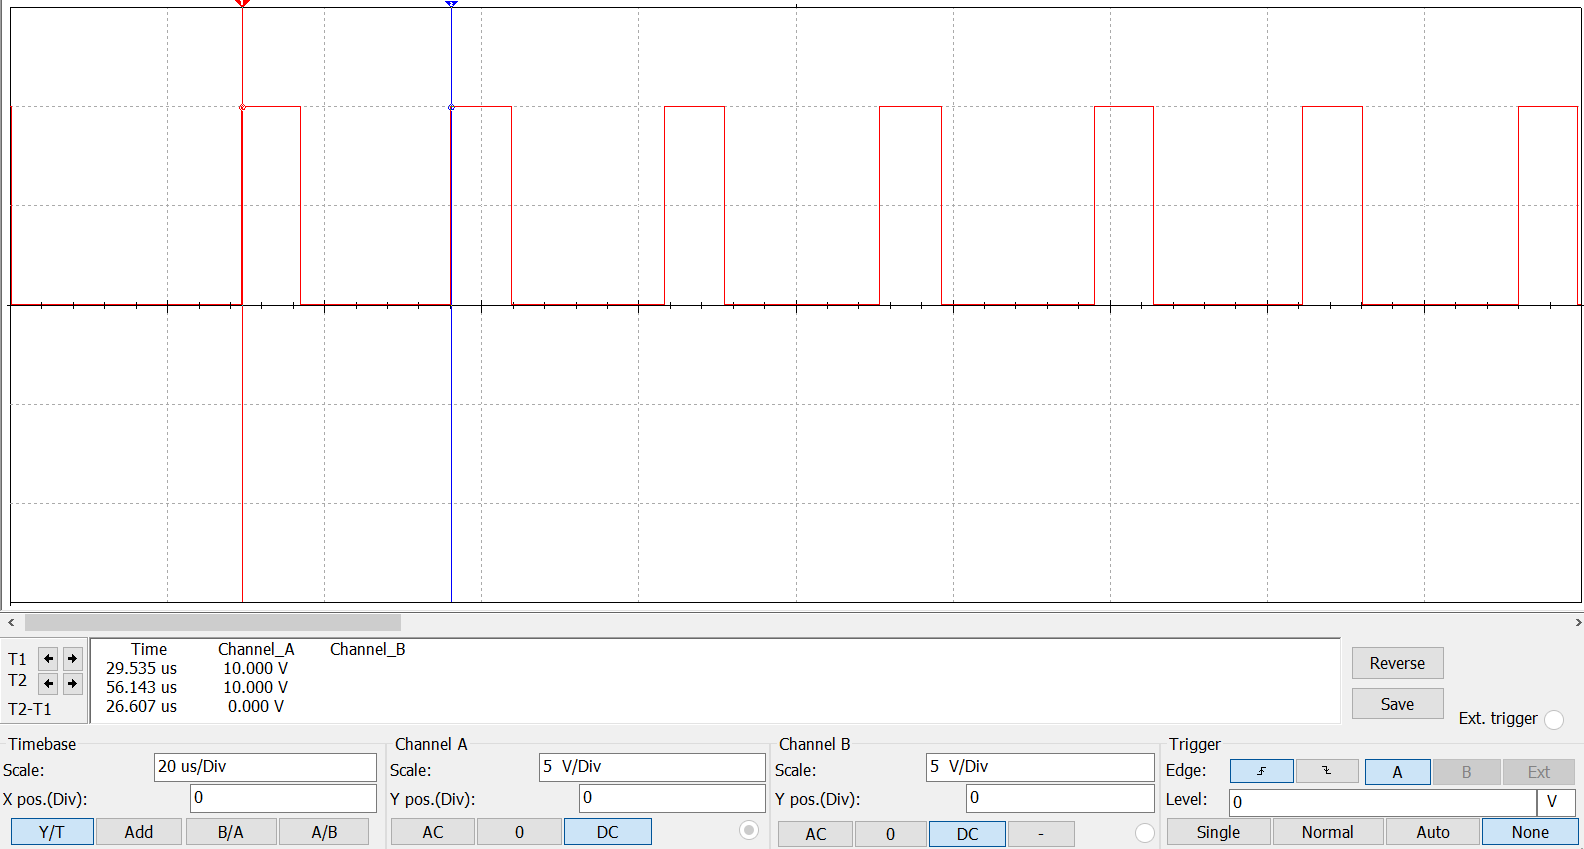
\includegraphics[width=0.8\textwidth]{4-4.png}
    \caption{红外发射周期}
    \label{fig:xfig1}
\end{figure}
\begin{figure}[H] % use float package if you want it here
    \centering
    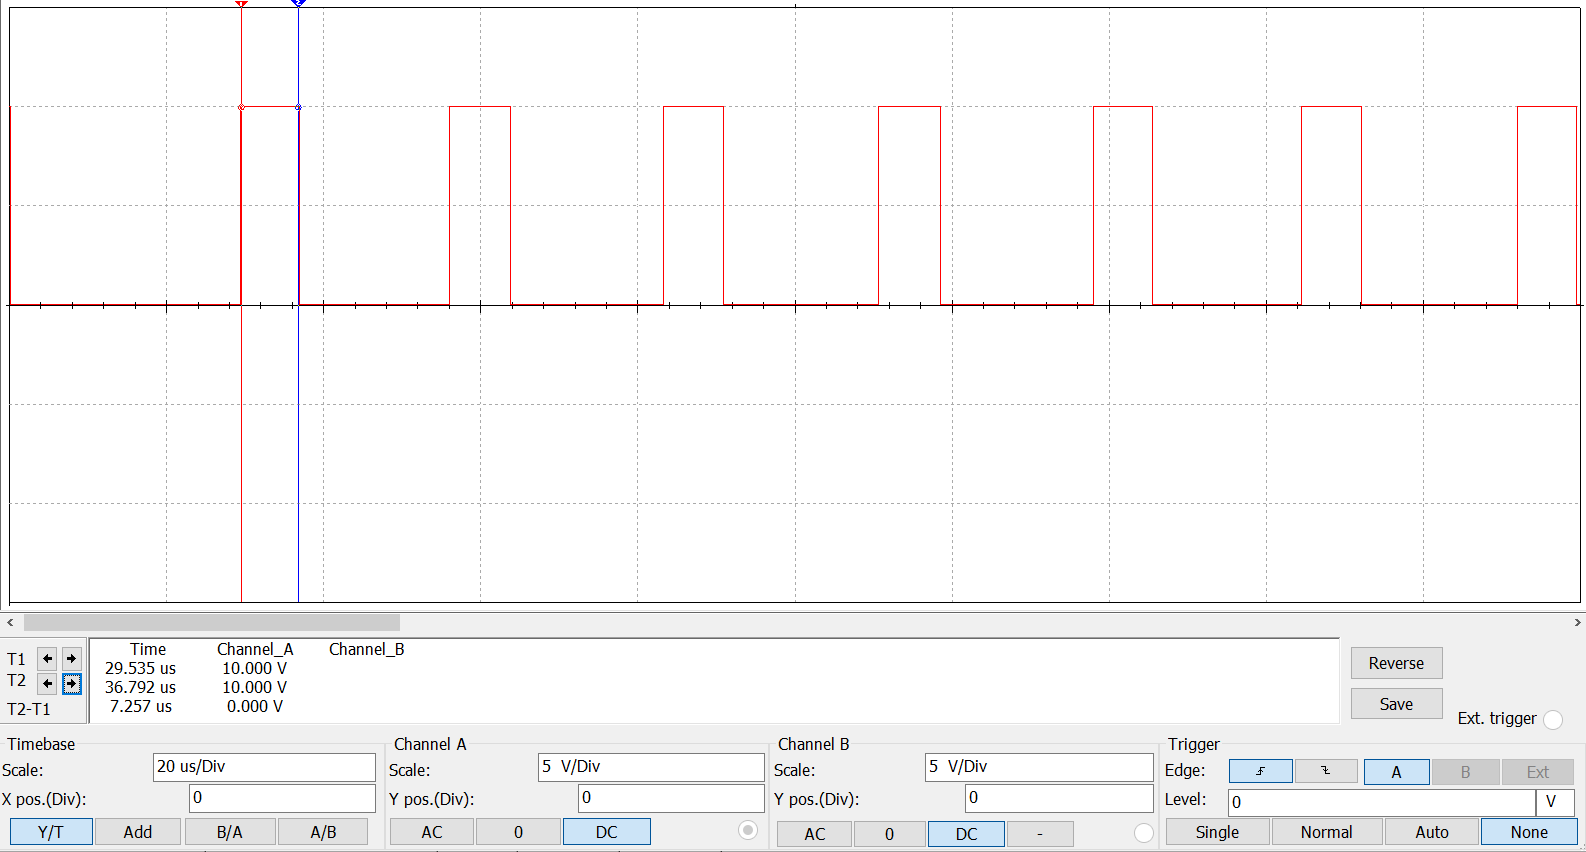
\includegraphics[width=0.8\textwidth]{4-5.png}
    \caption{红外发射占空比}
    \label{fig:xfig1}
\end{figure}



\section{红外接收Multisim仿真电路}
\begin{figure}[H] % use float package if you want it here
    \centering
    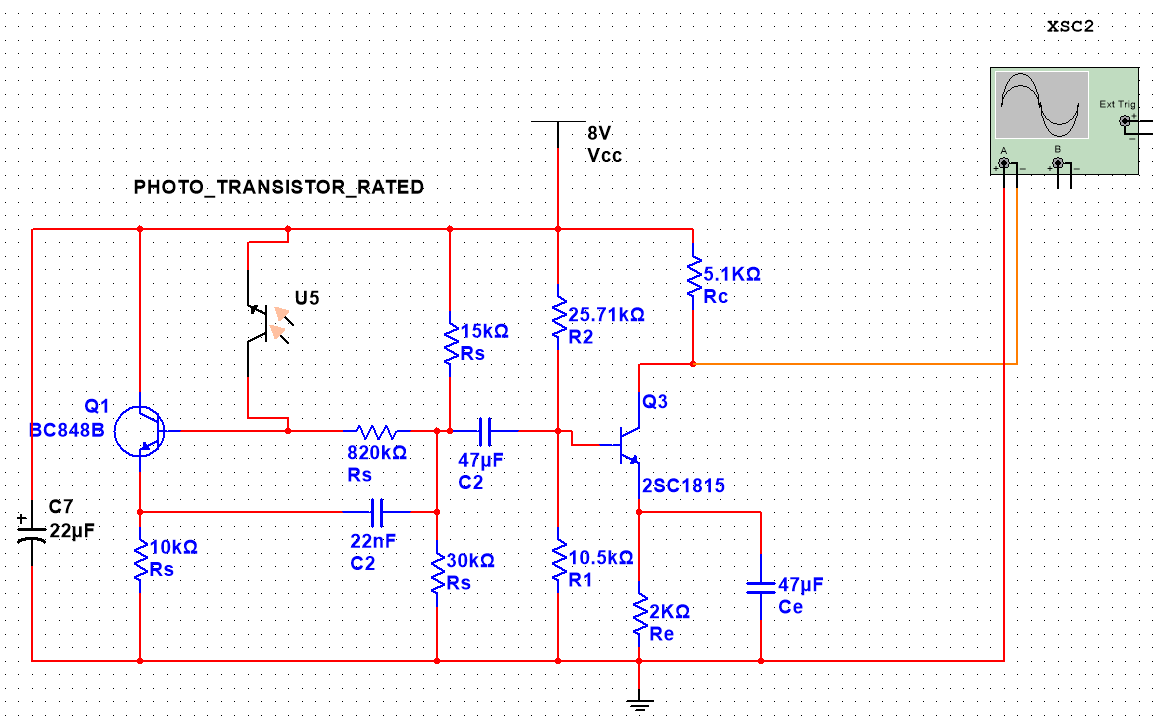
\includegraphics[width=1\textwidth]{5-1.png}
    \caption{红外接收Multisim仿真电路}
    \label{fig:xfig1}
\end{figure}

其中U5为发光二极管,其参数如下:

\begin{figure}[H] % use float package if you want it here
    \centering
    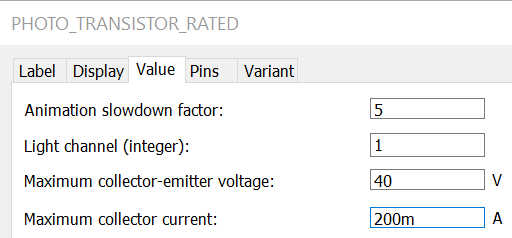
\includegraphics[width=0.5\textwidth]{5-2.png}
    \caption{U5参数}
    \label{fig:xfig1}
 \end{figure}

 ~\\

测量其输出电压波形如下:
\begin{figure}[H] % use float package if you want it here
    \centering
    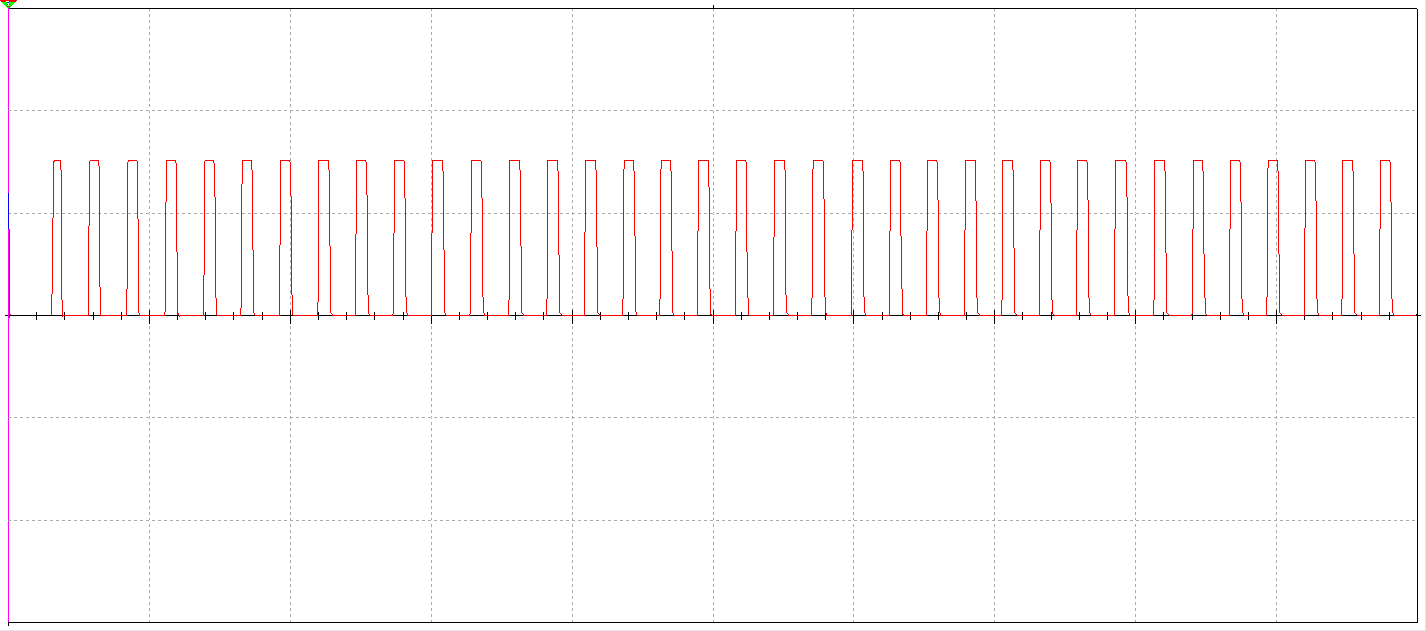
\includegraphics[width=0.8\textwidth]{5-3.png}
    \caption{红外接收整体波形}
    \label{fig:xfig1}
\end{figure}
\begin{figure}[H] % use float package if you want it here
    \centering
    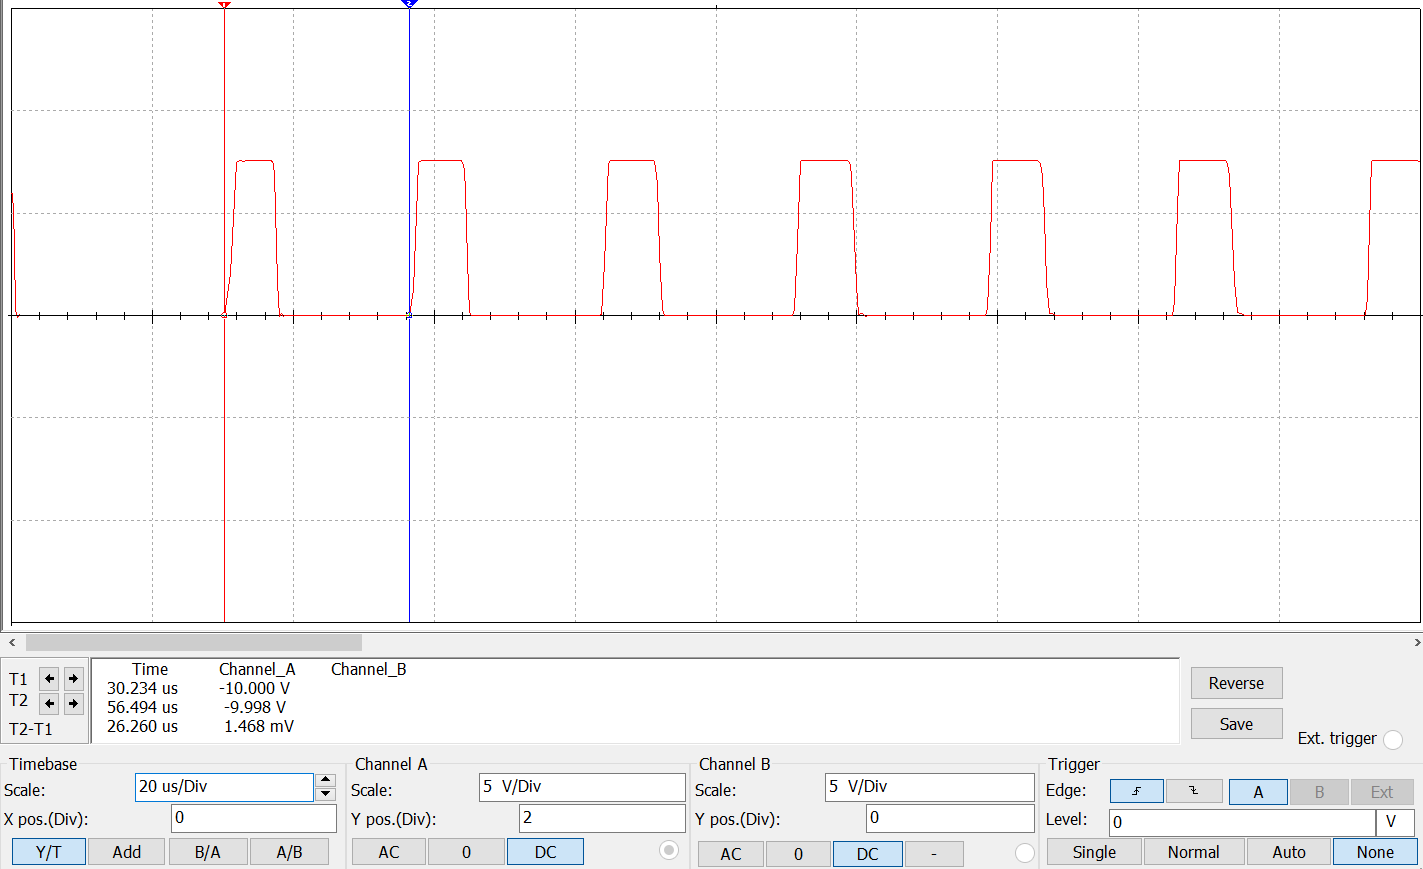
\includegraphics[width=0.8\textwidth]{5-4.png}
    \caption{红外接收周期}
    \label{fig:xfig1}
\end{figure}
\begin{figure}[H] % use float package if you want it here
    \centering
    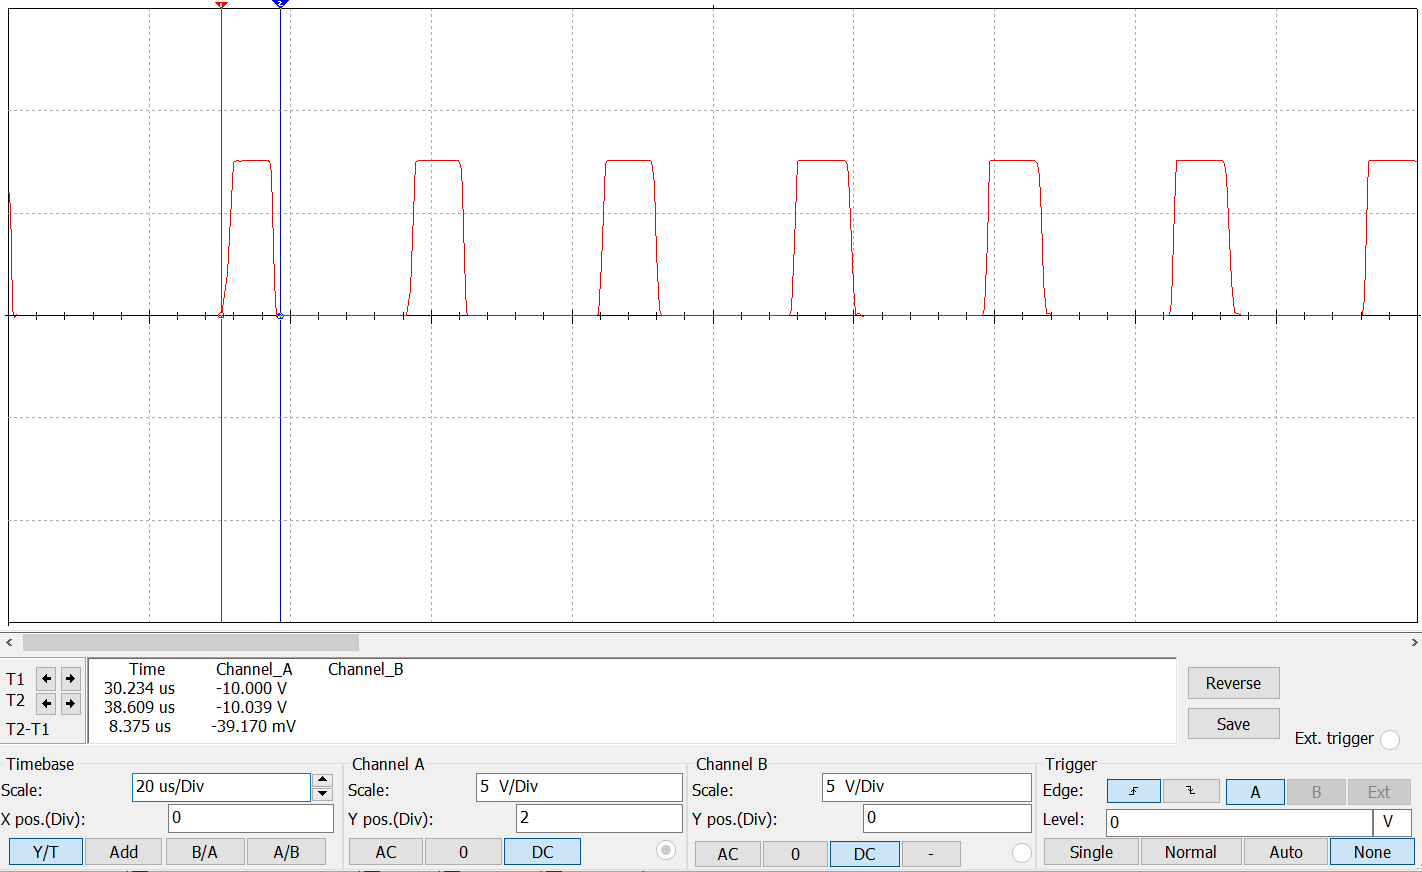
\includegraphics[width=0.8\textwidth]{5-5.png}
    \caption{红外接收占空比}
    \label{fig:xfig1}
\end{figure}

结果分析:\\
期望信号为38kHz、26.4\%占空比的方波。

实际红外发射信号周期为:26.607us,即频率为37.584kHz,误差为1.10\%

实际红外发射信号占空比为:7.257us/26.607us,即为27.27\%,误差为3.30\%

实际红外发射信号电压大小:10V

~\\

当以实际红外发射信号发射时,分析实际红外接收信号。

实际红外接收信号周期为:26.260us,即频率为38.08kHz,误差为1.30\%

实际红外接收信号占空比为:8.375us/26.260us,即为31.89\%,误差为16.94\%

实际红外接收信号电压大小:-20V,放大了-2倍

并且此时接收信号反映稍微的延时。因此实际占空比误差应该更小



均在误差允许范围之内,据此进行PCB的制作和设计结果分析。

\chapter{PCB}
\label{cha:intro}
通过仿真证明可以完整实现红外发射和接收任务,在此设计两块PCB板以将其实现。

\section{红外发射PCB板}
\begin{figure}[H] % use float package if you want it here
    \centering
    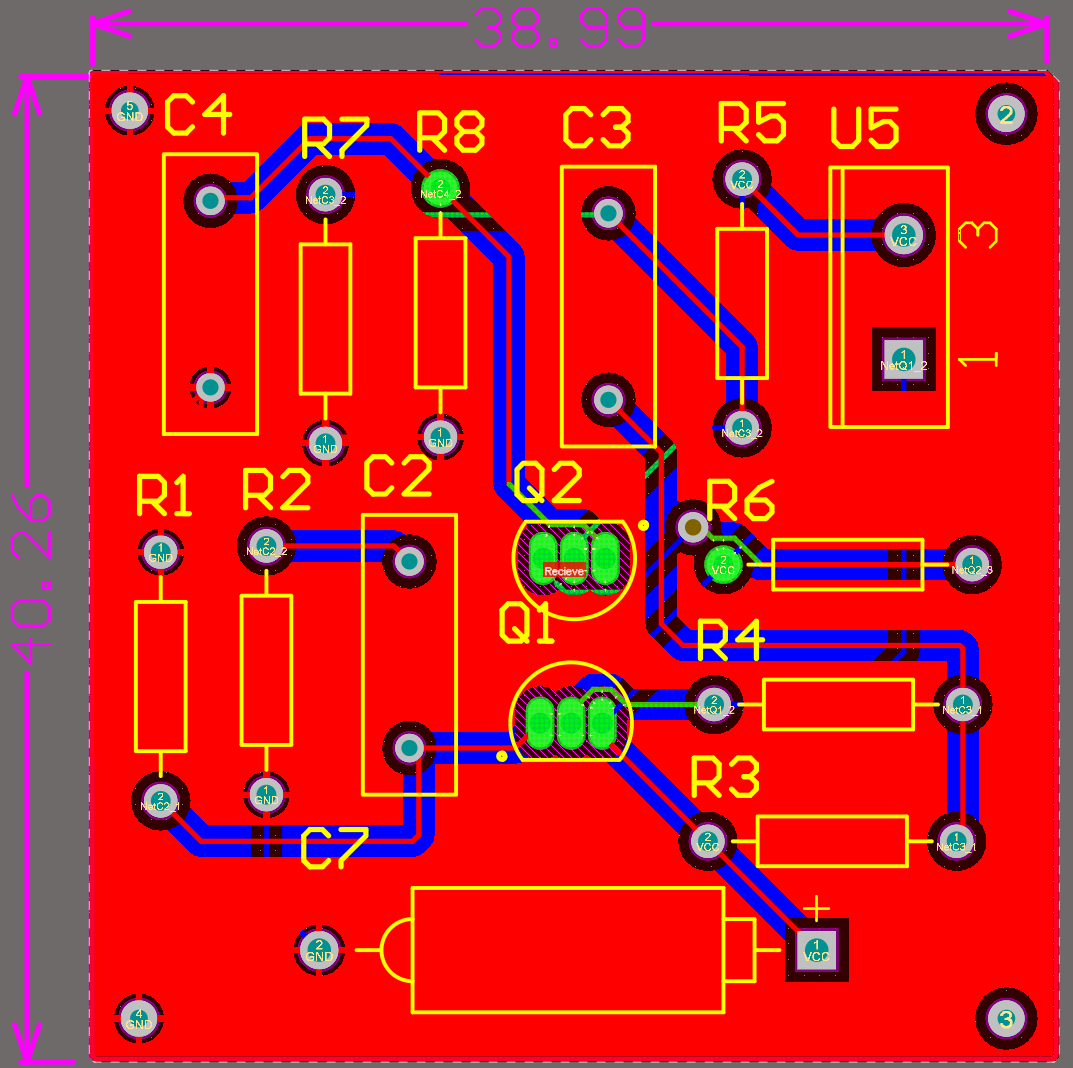
\includegraphics[width=1\textwidth]{6-1.png}
    \caption{Top Layer}
    \label{fig:xfig1}
\end{figure}

\begin{figure}[H] % use float package if you want it here
    \centering
    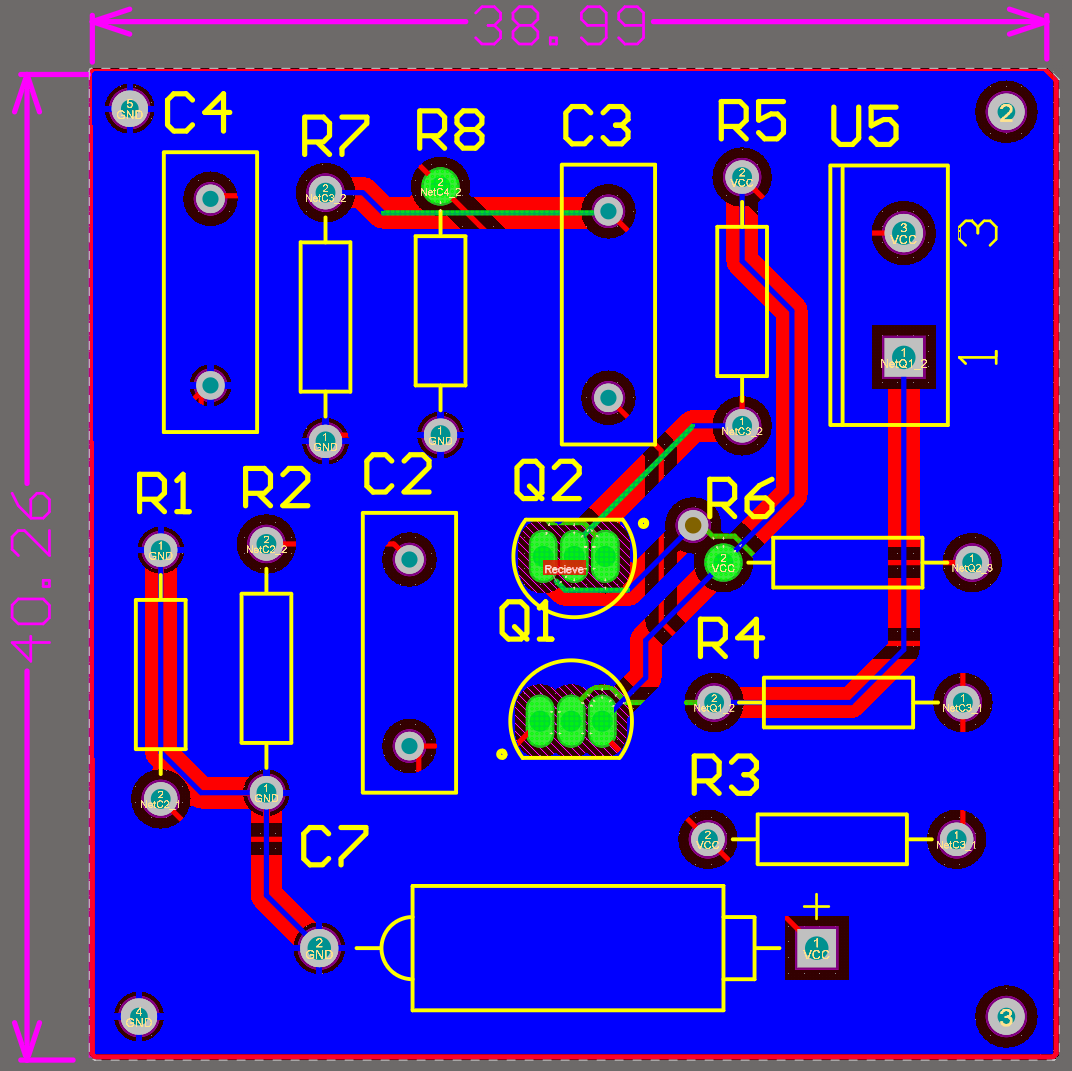
\includegraphics[width=1\textwidth]{6-3.png}
    \caption{Bottom Layer}
    \label{fig:xfig1}
 \end{figure}

 \section{红外接收PCB板}
 \begin{figure}[H] % use float package if you want it here
     \centering
     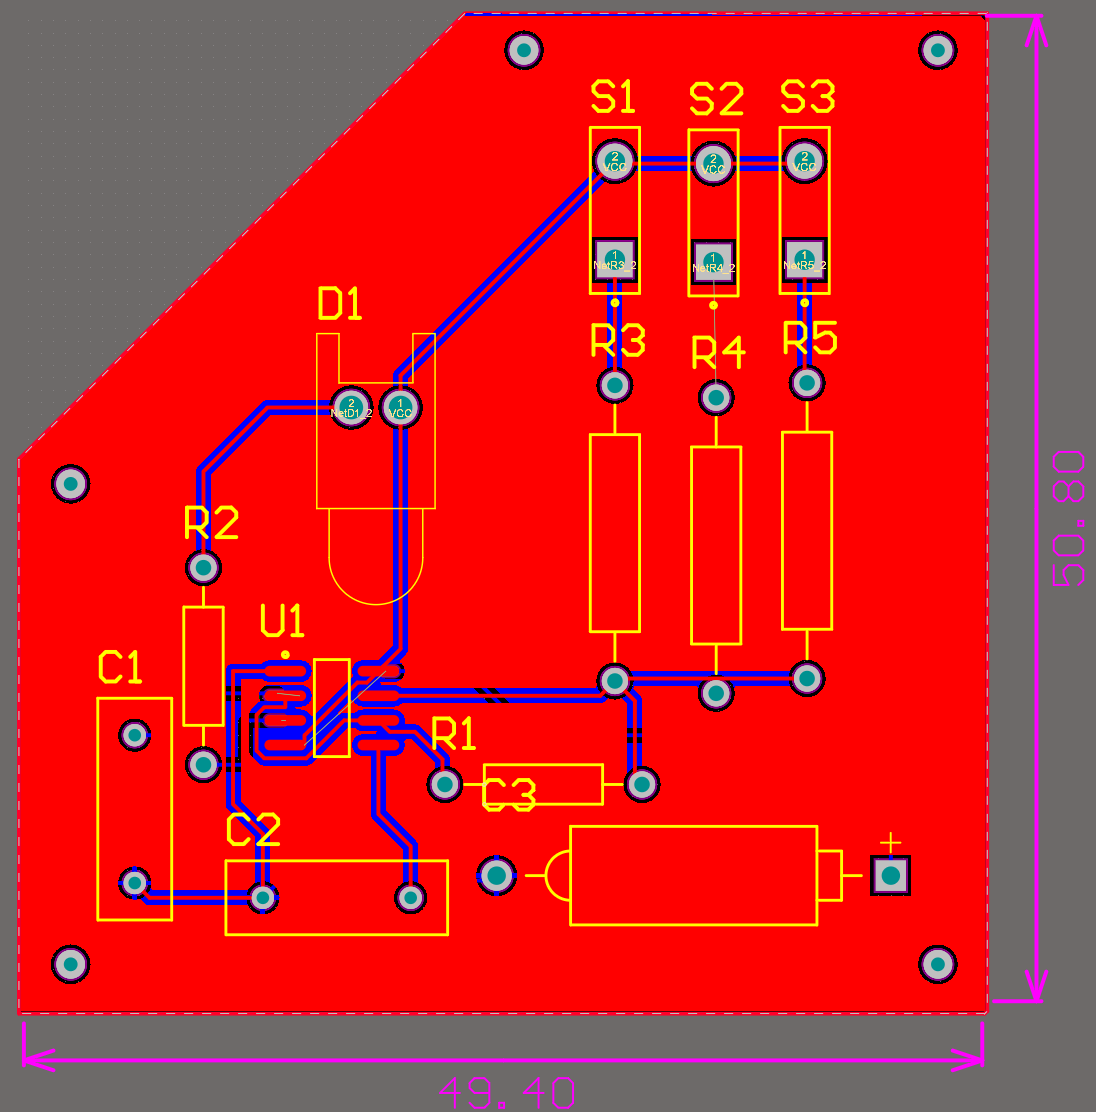
\includegraphics[width=1\textwidth]{6-2.png}
     \caption{Top Layer}
     \label{fig:xfig1}
 \end{figure}
 
 \begin{figure}[H] % use float package if you want it here
     \centering
     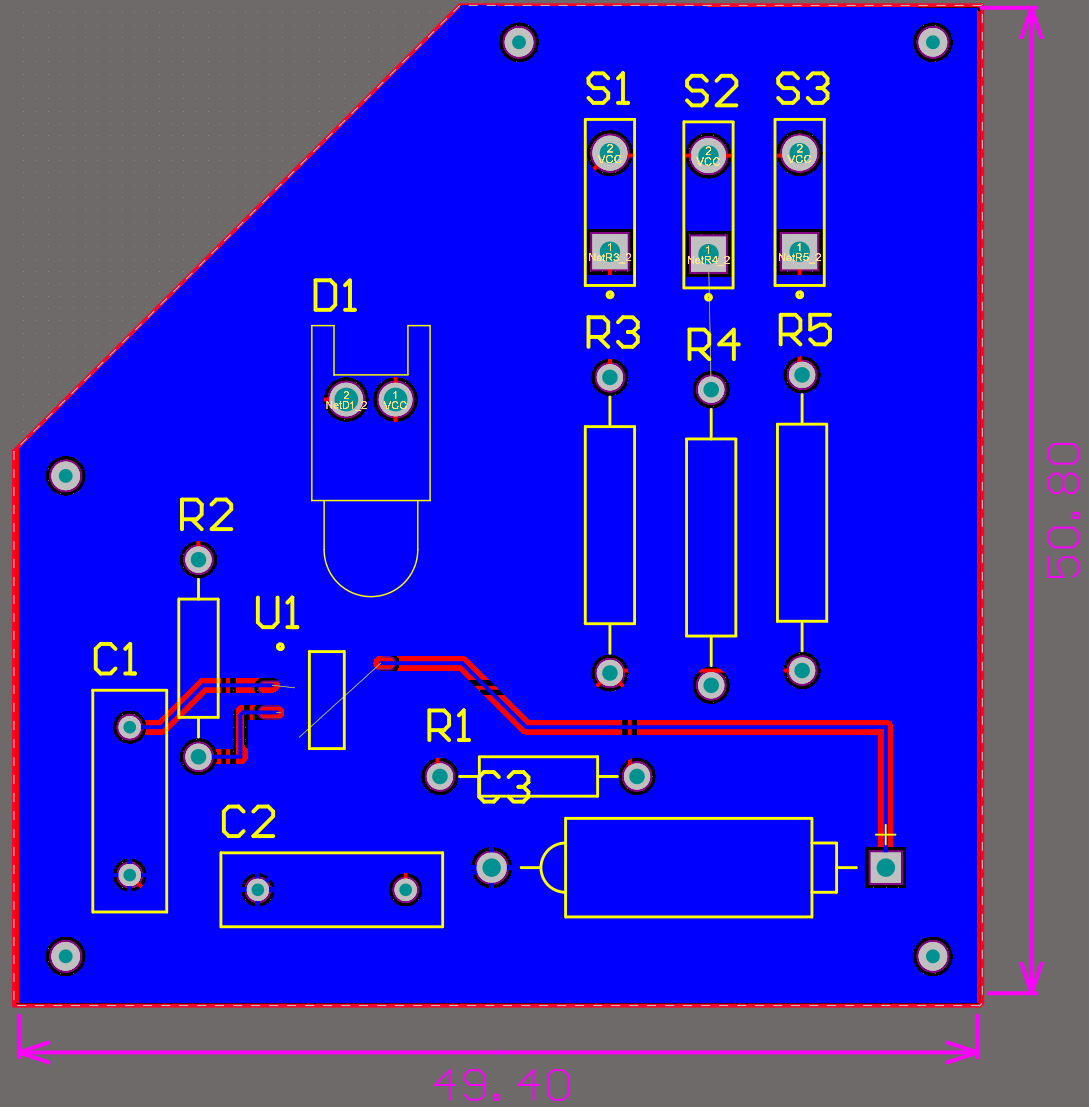
\includegraphics[width=1\textwidth]{6-4.png}
     \caption{Bottom Layer}
     \label{fig:xfig1}
  \end{figure}

\vspace{100pt}

\section{关键元器件参数}
NE555参数:
\begin{figure}[H] % use float package if you want it here
    \centering
    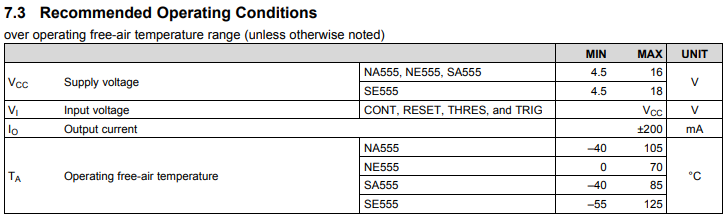
\includegraphics[width=1\textwidth]{NE555.png}
    \caption{NE555参数}
    \label{fig:xfig1}
 \end{figure}
 
2SC1815参数:
 \begin{figure}[H] % use float package if you want it here
     \centering
     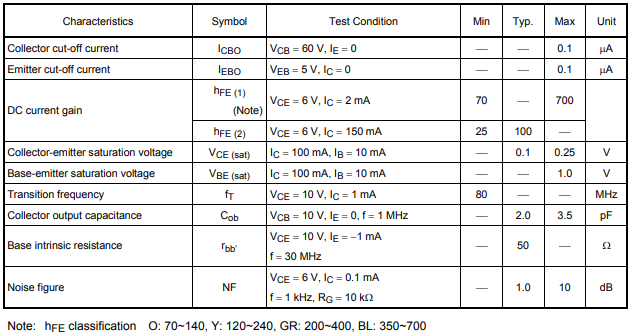
\includegraphics[width=1\textwidth]{2SC1815.png}
     \caption{2SC1815参数}
     \label{fig:xfig1}
  \end{figure}

BC848B参数:
\begin{figure}[H] % use float package if you want it here
    \centering
    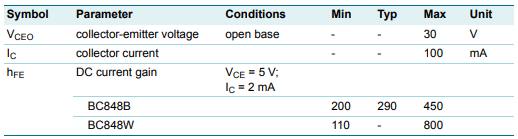
\includegraphics[width=1\textwidth]{BC848B.png}
    \caption{BC848B参数}
    \label{fig:xfig1}
 \end{figure}
\section{所有元器件列表}
\subsection{红外发射PCB板元器件列表}
\begin{figure}[H] % use float package if you want it here
    \centering
    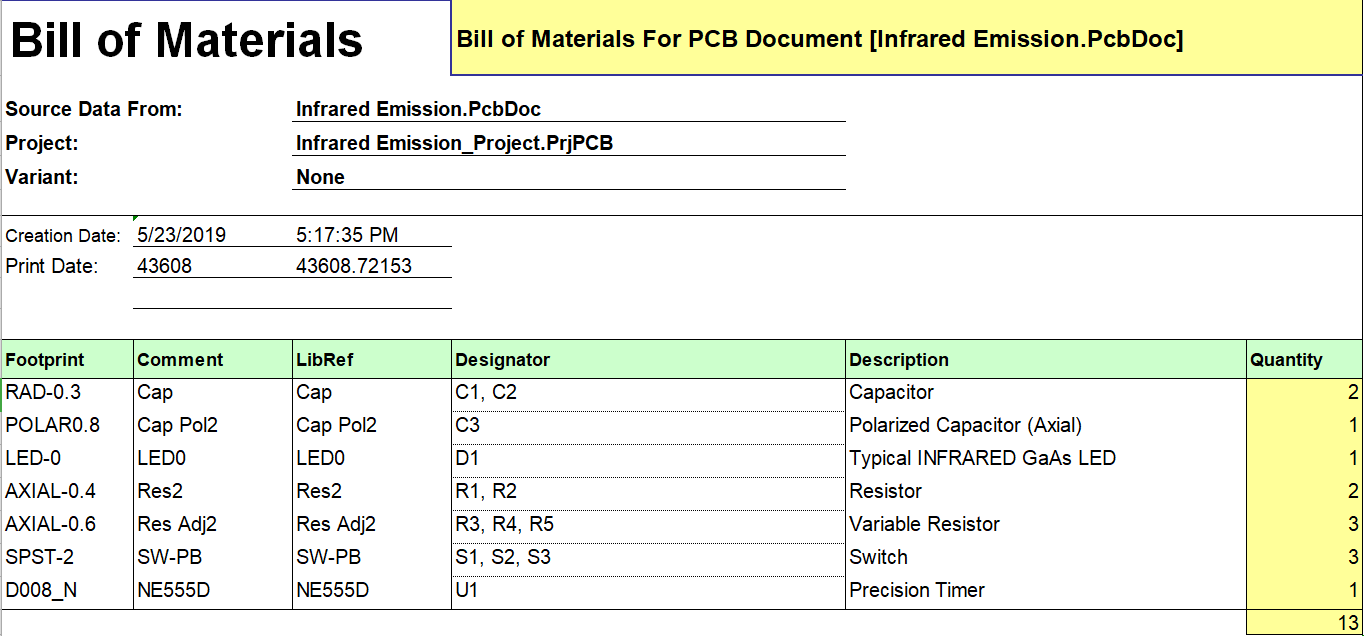
\includegraphics[width=1\textwidth]{7-1.png}
    \caption{红外发射PCB板元器件列表}
    \label{fig:xfig1}
 \end{figure}
\subsection{红外接收PCB板元器件列表}
\begin{figure}[H] % use float package if you want it here
    \centering
    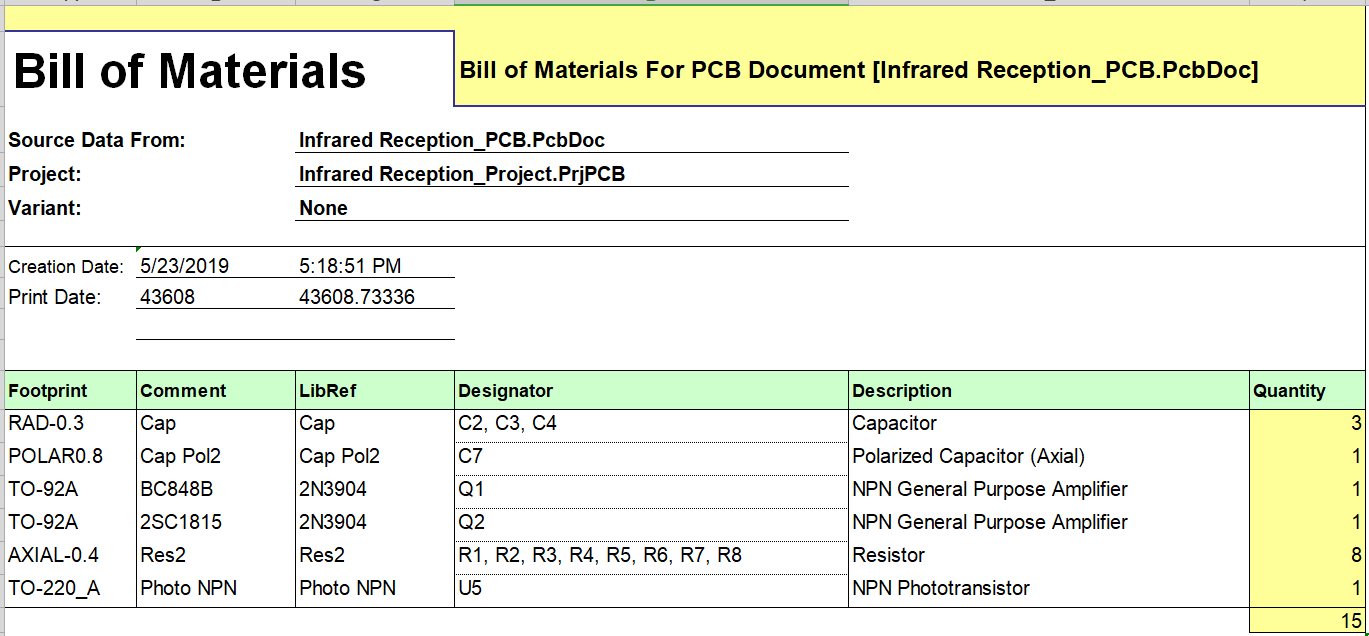
\includegraphics[width=1\textwidth]{7-2.png}
    \caption{红外接收PCB板元器件列表}
    \label{fig:xfig1}
 \end{figure}

 \subsection{管脚数量}
 \begin{figure}[H]
    \centering%
    \subcaptionbox{红外发射PCB板管脚数量\label{fig:subfig1}}[3cm] %标题的长度,超过则会换行,如下一个小图。
      {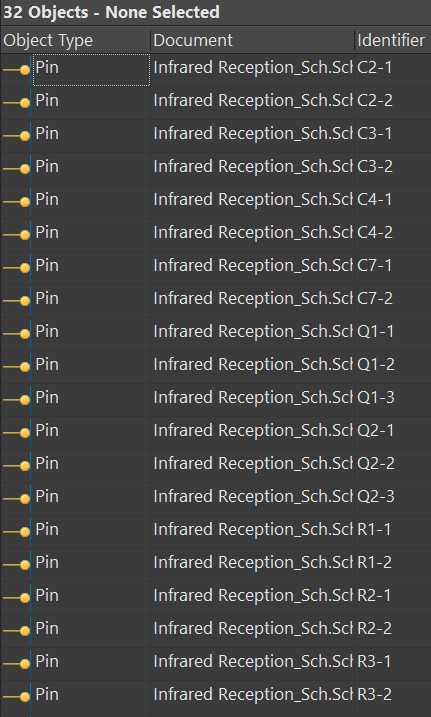
\includegraphics[width=0.3\textwidth]{8-1.png}}%
    \hspace{4em}%
    \subcaptionbox{红外接收PCB板管脚数量\label{fig:subfig2}}
        {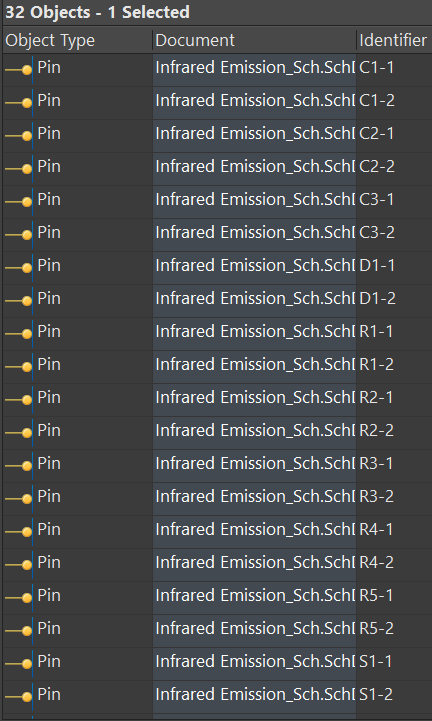
\includegraphics[width=0.3\textwidth]{8-2.png}}
    \caption{管脚数量}
    \label{fig:big1-subcaptionbox}
  \end{figure}
统计得到管脚数量为64根。

\subsection{进一步查看}

欢迎老师进行进一步的查看,附录中有\\

0. 论文写作的所有文件。以证明文章的原创性,需要使用Latex打开。
1. 原始版本的计划书\\
2. AD原理图以及PCB。里面有两个文件,分别时发射和接收,内有PCB和原理图源文件。\\
3. Multisim仿真及结果。里面有大量图片,均是仿真后的原图,文件需要使用Multisim14打开\\
4. 关键元器件手册。含有三个关键器件的芯片手册\\
非常希望老师能给出宝贵意见。随时可以联系我:812079716@qq.com。非常感谢老师!

\end{document}
